\documentclass[12pt]{article}

% --- Packages ---
\usepackage[T1]{fontenc}
\usepackage{lmodern}
\usepackage[margin=1in]{geometry}
\usepackage{amsmath,amssymb}
\usepackage{booktabs}
\usepackage{natbib}
\usepackage{float}
\usepackage{multirow}
\usepackage{graphicx}
\usepackage{hyperref}

\graphicspath{{figures/}}

\linespread{1.6}

\title{Occupational Skill Portability: A Gravity Model Approach with Applications to Unemployment and AI Displacement Risk}
\author{Jacob Guzman\thanks{University of San Francisco. Email: \texttt{jguzman14@dons.usfca.edu}.}}
\date{\today}

\begin{document}

\maketitle

\begin{abstract}
I construct a skill portability index for 525 U.S.\ occupations by estimating a gravity model of occupational switching using CPS data (2020--2025), O*NET skill profiles (202 dimensions), and commuting-zone employment distributions. Six candidate skill-distance measures, including three direct metrics and three machine-learning approaches, are evaluated comparatively. LASSO, which endogenously selects 117 of 202 O*NET dimensions, best predicts bilateral switching flows (pseudo-$R^2 = 0.478$). A fixed-exposure portability index derived from this model significantly predicts long-term unemployment across occupations ($\hat{\alpha}_2 = -0.0011$, $p = 0.008$): a one-standard-deviation increase in portability reduces the LTU share by 0.11 percentage points. Comparing LASSO-based and factor-analysis-based indices reveals that credentialed occupations, such as registered nurses (+202 ranks) and electricians (+303 ranks), are far more portable in latent skill space than observed switching suggests, consistent with licensing frictions suppressing mobility. AI exposure, measured via the Eloundou et al.\ (2023) scores, operates through an independent channel: the portability-LTU relationship survives conditioning on AI exposure ($p = 0.035$), and the interaction term is null ($p = 0.705$).
\end{abstract}

%=============================================================================
\section{Introduction}
\label{sec:intro}
%=============================================================================

A central question in labor economics is whether the skills a worker accumulates in one occupation transfer to others. When an occupation contracts due to trade shocks, technological displacement, or sectoral reallocation, workers' outside options depend critically on whether their human capital has value elsewhere in the labor market. Despite decades of research on human capital specificity \citep{becker1964,lazear2009}, the profession lacks a widely accepted, empirically validated measure of occupation-level skill portability.

Existing approaches to measuring skill overlap between occupations fall into two broad categories. The first imposes a single distance metric, typically Euclidean distance or cosine similarity, on a vector of skill descriptors, treating all dimensions as equally relevant to mobility \citep{poletaev2008,gathmann2010}. This assumption may be overly restrictive: some dimensions (e.g., broad cognitive abilities) are widely shared and plausibly drive transitions, while narrow knowledge categories used by only a few occupations may contribute little to observed mobility. The second category relies on ad-hoc skill taxonomies that aggregate detailed descriptors into a handful of predetermined categories, discarding within-category variation.

This paper proposes an alternative: let observed worker switching behavior reveal which skill dimensions constrain mobility. I estimate a gravity model of bilateral occupational switching in the spirit of trade gravity models, where the ``flow'' between two occupations depends on their skill distance, geographic overlap, origin size, and destination labor demand. The key methodological innovation is a comparative evaluation of six candidate skill-distance measures: three based on direct formulas (Euclidean, angular separation, factor analysis) and three based on machine-learning models (LASSO, Random Forest, XGBoost) that are trained to predict switching from per-dimension O*NET skill differences. Cross-validated out-of-fold predictions ensure that the ML-based distances do not mechanically overfit.

The preferred specification, LASSO estimated via Pseudo Poisson Maximum Likelihood (PPML), achieves a pseudo-$R^2$ of 0.478, with geographic distance contributing an additional 9.8 percentage points of explanatory power. LASSO endogenously selects 117 of 202 O*NET dimensions, effectively learning which skills constrain mobility rather than treating all dimensions symmetrically. To aggregate pair-level predictions into a single portability score per occupation, I adopt a fixed-exposure specification that strips origin-size contamination from the predicted switching rates, then rank-normalize the employment-share-weighted rates to a $[0,1]$ index.

The portability index is validated against long-term unemployment (LTU). In the original specification with free exposure, portability does not predict LTU ($p = 0.279$). The fixed-exposure index, however, significantly predicts LTU ($\hat{\alpha}_2 = -0.0011$, $p = 0.008$, 95\% CI $[-0.0019, -0.0003]$): a one-standard-deviation increase in portability reduces the LTU share by 0.11 percentage points. The sign flip, from positive (nonsensical) to negative (theory-consistent), underscores the importance of stripping origin-size contamination from the index.

Comparing the LASSO-based index with a factor-analysis-based alternative reveals a substantively important divergence. The two indices correlate at $\rho = 0.890$ overall, but disagree sharply on credentialed occupations: registered nurses rank 202 positions higher under factor analysis (rank 47 vs.\ 249), and electricians rank 303 positions higher (rank 95 vs.\ 398). Factor analysis captures latent structural transferability, the broad skill overlap that \emph{could} support transitions, while LASSO captures revealed transferability conditional on observed switching. The divergence maps onto known licensing frictions: these occupations' skill profiles overlap with many large destinations, but credentialing barriers suppress realized mobility.

Finally, I incorporate AI exposure using the \citet{eloundou2023} scores. Portability remains significant after controlling for AI exposure ($p = 0.035$), the interaction between portability and AI exposure is null ($p = 0.705$), and subsample splits by AI exposure level show similar portability coefficients in both halves. The portability--LTU channel is independent of AI displacement risk.

This paper contributes to several literatures. Relative to \citet{gathmann2010}, who measure task distance between occupations and show it predicts wage losses upon switching, I validate the distance measure not just against switching \emph{behavior} but against a downstream labor market \emph{outcome} (LTU). Relative to \citet{poletaev2008}, who show skill mismatch reduces wages after displacement, I allow the data to weight skill dimensions endogenously rather than imposing predetermined categories. The comparison of factor-analysis and LASSO indices connects to \citet{kleiner2013} on licensing frictions and to \citet{lazear2009} on skill specificity. The AI exposure analysis contributes to the growing literature on technology-driven labor reallocation \citep{cortes2018,autor2013}.

The remainder of the paper is organized as follows. Section \ref{sec:data} describes the data sources. Section \ref{sec:strategy} presents the empirical strategy. Section \ref{sec:results} reports results. Section \ref{sec:discussion} discusses interpretation and limitations. Section \ref{sec:conclusion} concludes.

%=============================================================================
\section{Data}
\label{sec:data}
%=============================================================================

The analysis combines five data sources: occupational switching counts from the Current Population Survey, skill profiles from O*NET, geographic employment distributions from the American Community Survey, job openings from Lightcast, and AI exposure scores from \citet{eloundou2023}. All occupation-level variables are defined at the Census 2018 four-digit occupation code level, which serves as the common identifier throughout the pipeline.

%-----------------------------------------------------------------------------
\subsection{Occupational Switching (CPS ASEC 2020--2025)}
\label{sec:data_cps}
%-----------------------------------------------------------------------------

Bilateral switching counts come from the Annual Social and Economic Supplement (ASEC) of the Current Population Survey (CPS), accessed via IPUMS, for survey years 2020--2025. A respondent is classified as a \emph{switcher} if their current occupation code (\texttt{OCC}) differs from their prior-year occupation code (\texttt{OCCLY}). The sample is restricted to employed persons (EMPSTAT 10 or 12), ages 16--64, who are ASEC respondents (ASECFLAG $> 0$). Switching counts are raw person totals, unweighted, pooled across all six years to maximize sample size.

This procedure identifies 525 occupations, 275,100 directed occupation pairs, of which 13,756 (5.0\%) have at least one observed switch, and 47,770 total switchers. The individual-level switching rate is 12.5\%, which is high relative to the $\sim$5\% benchmark in the literature \citep{kambourov2008}. The inflation likely reflects occupation coding error in the CPS: respondents report occupation titles that are then coded independently in consecutive surveys, so spurious switches arise from inconsistent coding rather than genuine job changes. This measurement error attenuates the relationship between skill distance and switching but does not bias the coefficient toward significance, making it a conservative concern for our main results.

%-----------------------------------------------------------------------------
\subsection{Skill Profiles (O*NET 30.1)}
\label{sec:data_onet}
%-----------------------------------------------------------------------------

Skill profiles are drawn from the Occupational Information Network (O*NET) database, version 30.1. I use four descriptor files: Skills (35 dimensions), Abilities (52 dimensions), Knowledge (33 dimensions), and Work Activities (41 activities $\times$ 2 scales for level and importance, yielding 82 dimensions), for a total of 202 numeric dimensions per occupation. Each dimension is filtered to the Level scale (and Importance scale for Work Activities), excluding suppressed ratings (\texttt{Recommend Suppress = ``N''}). O*NET-SOC codes are truncated to six-digit SOC, values are averaged within each SOC, and all dimensions are min-max normalized to $[0,1]$.

The resulting skill matrix (774 SOC codes $\times$ 202 dimensions) is mapped to Census 2018 occupation codes via the Census Bureau's 2018 occupation crosswalk. For each Census code, the crosswalk provides one or more SOC codes; when multiple SOCs map to a single Census code (typically for ``all other'' residual categories), the O*NET vectors are averaged. The match rate is 565 of 568 Census codes (99.5\%), with only three military codes unmatched. Approximately 93\% of mappings are exact one-to-one SOC matches; the remaining 7\% are residual categories resolved via wildcard or prefix matching.

%-----------------------------------------------------------------------------
\subsection{Geographic Distance (ACS 2021 + Dorn CZ Crosswalk)}
\label{sec:data_geo}
%-----------------------------------------------------------------------------

Geographic distance is measured as the Duncan dissimilarity index of commuting-zone (CZ) employment shares between occupation pairs. The Duncan index is a standard measure of spatial segregation, bounded in $[0,1]$, where 0 indicates identical geographic distributions and 1 indicates complete spatial disjointness.

Employment by occupation and commuting zone is computed from the American Community Survey (ACS) 2021 one-year file via IPUMS. The ACS provides person-level records with occupation codes and geographic identifiers (state, PUMA). PUMAs are mapped to commuting zones using the \citet{dorn2009} crosswalk, originally constructed for \citet{autor2013}.\footnote{The crosswalk uses 2010-vintage PUMA boundaries. ACS 2022 and later use 2020-vintage PUMAs, which are incompatible with this crosswalk. ACS 2021 is therefore the most recent compatible year. Geographic employment distributions evolve slowly, so 2021 is a reasonable proxy for the 2023 reference year specified in the research design.} Each person-CZ observation is weighted by the ACS person weight times the PUMA-to-CZ allocation factor. The resulting geographic distance matrix covers all 275,100 pairs in the analysis, with values ranging from 0.10 to 1.00 (mean = 0.65).

Commuting zones, as defined by \citet{tolbert1996} and updated by \citet{dorn2009}, approximate local labor markets by grouping counties according to commuting patterns. They are preferred to states (too large to capture local labor markets) and to counties (too small and numerous for meaningful occupation-level employment counts).

%-----------------------------------------------------------------------------
\subsection{Job Openings (Lightcast 2023)}
\label{sec:data_openings}
%-----------------------------------------------------------------------------

Destination labor demand is measured as each occupation's share of total job postings, computed from Lightcast (formerly Burning Glass Technologies) data for calendar year 2023. Total postings are summed by SOC 2021 five-digit code across months, then mapped to Census 2018 codes via the Census occupation crosswalk. The match rate is 655 of 657 SOC codes (99.7\%), covering 98.1\% of all 2023 postings, yielding openings shares for 520 Census occupation codes.

%-----------------------------------------------------------------------------
\subsection{AI Exposure (Eloundou et al.\ 2023)}
\label{sec:data_ai}
%-----------------------------------------------------------------------------

AI exposure scores come from \citet{eloundou2023}, who assess each occupation's exposure to large language models (specifically GPT-4) using a combination of human annotation and model-based scoring. The ``beta'' scores, which capture the share of occupation tasks that could be significantly accelerated by LLM access, are mapped to Census 2018 codes. These scores are used as a control variable and interaction term in the LTU validation regressions.

%-----------------------------------------------------------------------------
\subsection{Summary Statistics}
\label{sec:data_summary}
%-----------------------------------------------------------------------------

Table \ref{tab:summary} summarizes the key dimensions of the analysis dataset.

\begin{table}[H]
\centering
\caption{Summary Statistics}
\label{tab:summary}
\begin{tabular}{lr}
\toprule
\textbf{Dimension} & \textbf{Value} \\
\midrule
Occupations & 525 \\
Directed pairs & 275,100 \\
Pairs with nonzero switches & 13,756 (5.0\%) \\
Total switchers (pooled 2020--2025) & 47,770 \\
Individual-level switching rate & 12.5\% \\
O*NET skill dimensions & 202 \\
Commuting zones & 741 \\
Census--O*NET match rate & 565/568 (99.5\%) \\
Lightcast--Census match rate & 655/657 (99.7\%) \\
\bottomrule
\end{tabular}
\end{table}

Figure \ref{fig:switching_dist} illustrates the distributional features of the switching data that motivate the choice of estimator. Panel (a) shows that 95\% of directed occupation pairs have zero observed switches, creating a dominant extensive margin. Panel (b) shows that conditional on any switching, the distribution is heavily right-skewed: the median pair has just one observed switch, while a few high-flow pairs have over 100. Both features favor PPML over OLS.

\begin{figure}[H]
\centering
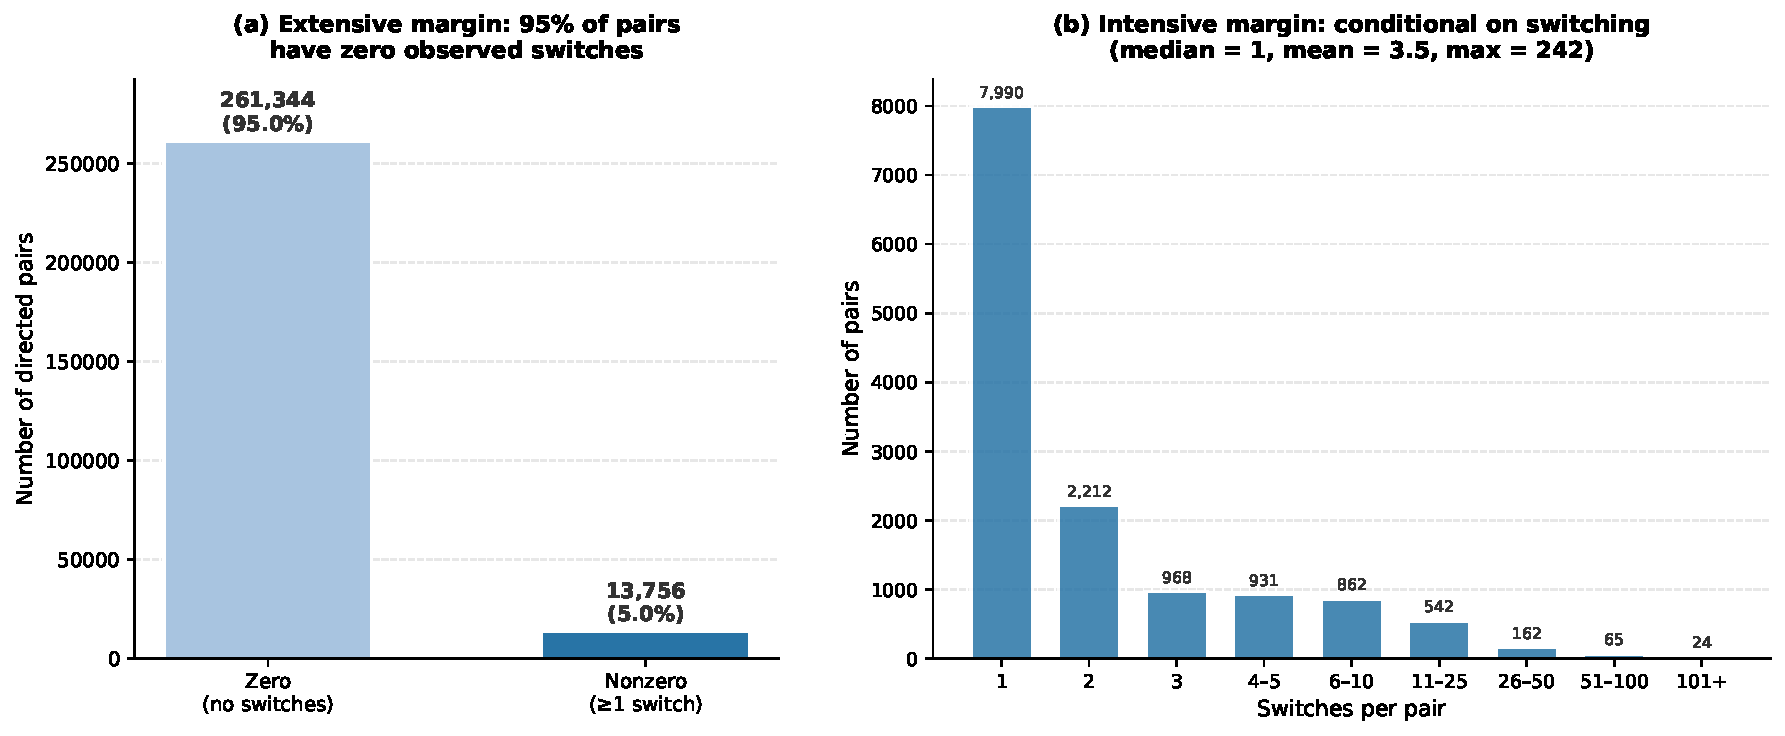
\includegraphics[width=\textwidth]{fig_switching_distribution.pdf}
\caption{Distribution of bilateral switching counts across 275,100 directed occupation pairs. Panel (a): extensive margin. Panel (b): intensive margin, conditional on at least one observed switch.}
\label{fig:switching_dist}
\end{figure}

%=============================================================================
\section{Empirical Strategy}
\label{sec:strategy}
%=============================================================================

The empirical strategy proceeds in two stages. The first stage constructs a validated skill portability index by estimating a gravity model of bilateral occupational switching, evaluating six candidate skill-distance measures, and aggregating pair-level predictions into a single score per occupation. The second stage tests whether this portability score predicts long-term unemployment across occupations.

%-----------------------------------------------------------------------------
\subsection{The Switching Model}
\label{sec:strategy_model}
%-----------------------------------------------------------------------------

The baseline specification is a gravity model of labor mobility:
\begin{equation}
\label{eq:switching}
\text{Switches}_{o,d} = \beta_0 + \beta_1 \, \text{SkillDistance}_{o,d} + \beta_2 \, \text{GeographicDistance}_{o,d} + \delta_1 \, \text{Switches}_{o,d^*} + \delta_2 \, \text{OpeningsShare}_d + \nu_{o,d}
\end{equation}
where $\text{Switches}_{o,d}$ is the raw count of CPS respondents who switched from occupation $o$ to occupation $d$ over the pooled 2020--2025 window; $\text{SkillDistance}_{o,d}$ is a measure of skill dissimilarity between the origin and destination (defined below); $\text{GeographicDistance}_{o,d}$ is the Duncan overlap index between the two occupations' CZ employment distributions; $\text{Switches}_{o,d^*} = \sum_{d'} \text{Switches}_{o,d'}$ is the total number of switchers out of origin $o$; and $\text{OpeningsShare}_d$ is the destination's share of national job postings.

The controls $\delta_1$ and $\delta_2$ are essential. Without them, skill distance would appear to predict switching partly because it correlates with origin and destination size. A large occupation mechanically generates more bilateral flows to every destination; a high-demand destination absorbs more flows from every origin. The controls net out these mechanical effects, isolating the \emph{pair-specific excess switching} attributable to skill similarity ($\beta_1$) and geographic co-location ($\beta_2$).

Equation (\ref{eq:switching}) is estimated by two methods. \textbf{OLS on $\log(1 + \text{Switches}_{o,d})$} is standard but distorts the extensive margin: the $+1$ transform compresses variation among zeros and positives. \textbf{Pseudo Poisson Maximum Likelihood (PPML)}, following \citet{santos2006}, is the preferred estimator. PPML is consistent for multiplicative models with heteroskedasticity and many zeros, both features of the switching data, where 95\% of pairs have zero observed switches. In the results, PPML substantially outperforms OLS ($R^2 = 0.478$ vs.\ $0.196$ for the best specification).

%-----------------------------------------------------------------------------
\subsection{Skill Distance Measures}
\label{sec:strategy_skill}
%-----------------------------------------------------------------------------

Six candidate skill-distance measures are constructed from the 202-dimensional O*NET skill vectors:

\paragraph{Direct metrics.} Three measures compute distance directly from the skill vectors:
\begin{enumerate}
    \item \textbf{Euclidean distance}: the $L_2$ norm of the difference vector between origin and destination skill profiles.
    \item \textbf{Angular separation}: $\arccos\!\bigl(\text{cosine similarity}(s_o, s_d)\bigr)$, which captures the angle between skill vectors regardless of magnitude.
    \item \textbf{Factor analysis}: Euclidean distance in a four-factor space obtained by fitting a factor model to all 565 occupation skill vectors. This compresses the 202 dimensions into four latent factors before computing distance.
\end{enumerate}

\paragraph{ML-based metrics.} Three measures are \emph{trained} to predict bilateral switches from per-dimension skill differences:
\begin{enumerate}
    \setcounter{enumi}{3}
    \item \textbf{LASSO}: LassoCV with five-fold cross-validation on 202 per-dimension absolute differences ($|s_o^{(k)} - s_d^{(k)}|$ for each dimension $k$). Out-of-fold predictions serve as the skill distance. LASSO selects 117 of 202 nonzero coefficients.
    \item \textbf{Random Forest}: 100 trees, max depth 12, minimum 50 samples per leaf. Five-fold out-of-fold predictions.
    \item \textbf{XGBoost}: 200 trees, learning rate 0.05, subsample 0.8. Five-fold out-of-fold predictions.
\end{enumerate}

For each ML model, the ``skill distance'' for a pair is that model's predicted switch count given only the O*NET skill differences as input. The full model (Equation \ref{eq:switching}) then tests how well this skill-based prediction explains actual switches after controlling for geographic distance, origin size, and destination openings. The use of cross-validated out-of-fold predictions prevents the ML-based distances from mechanically overfitting to the dependent variable.

Running Equation (\ref{eq:switching}) separately for each of the six skill-distance variants under both OLS and PPML produces twelve specifications. The variant with the highest $R^2$ in the preferred PPML estimator is selected for index construction.

%-----------------------------------------------------------------------------
\subsection{Geographic Distance}
\label{sec:strategy_geo}
%-----------------------------------------------------------------------------

Geographic distance between occupations $o$ and $d$ is the Duncan dissimilarity index:
\begin{equation}
\label{eq:duncan}
\text{GeographicDistance}_{o,d} = \frac{1}{2} \sum_{c} \left| \text{EmpShare}_{o,c} - \text{EmpShare}_{d,c} \right|
\end{equation}
where $c$ indexes commuting zones and
\begin{equation}
\label{eq:empshare}
\text{EmpShare}_{o,c} = \frac{\text{emp}_{o,c}}{\text{emp}_o}
\end{equation}
is occupation $o$'s share of employment in commuting zone $c$. The index equals zero when both occupations have identical geographic distributions (a worker in $o$ can access $d$ without relocating) and approaches one when they are spatially disjoint.

%-----------------------------------------------------------------------------
\subsection{Portability Index Construction}
\label{sec:strategy_index}
%-----------------------------------------------------------------------------

The portability index aggregates pair-level model predictions into a single score per occupation. The baseline aggregation (Equations 5--6 in the research design) is:
\begin{equation}
\label{eq:portability}
\text{Portability}_o = \sum_{d} \omega_d \cdot \hat{y}_{o,d}, \qquad \omega_d = \text{EmpShare}_d
\end{equation}
where $\hat{y}_{o,d}$ is the fitted value from Equation (\ref{eq:switching}) and $\text{EmpShare}_d$ is destination $d$'s share of national employment. This computes an employment-weighted average of predicted switches from origin $o$ to all destinations, giving higher weight to destinations that represent larger shares of the labor market.

\paragraph{The origin-size contamination problem.} When $\delta_1$ is estimated freely, the fitted value $\hat{y}_{o,d}$ scales positively with $\text{Switches}_{o,d^*}$ (total switches out of origin $o$). Aggregating $\hat{y}$ across destinations therefore makes large origins mechanically score higher, regardless of their structural skill transferability. This produces counterintuitive rankings: cashiers and retail workers dominate the top, while software developers and registered nurses, occupations with arguably broad, transferable skills, cluster at the bottom.

\paragraph{The fixed-$\delta_1$ exposure solution.} To isolate structural transferability, I re-estimate Equation (\ref{eq:switching}) with $\delta_1$ fixed to 1 by entering $\text{Switches}_{o,d^*}$ as a PPML exposure term:
\begin{equation}
\label{eq:exposure}
E[\text{Switches}_{o,d} \mid X] = \text{Switches}_{o,d^*} \cdot \exp\!\bigl(\beta_0 + \beta_1 \, \text{SkillDist}_{o,d} + \beta_2 \, \text{GeoDist}_{o,d} + \delta_2 \, \text{OpeningsShare}_d\bigr)
\end{equation}
The predicted \emph{rate per switcher},
\begin{equation}
\label{eq:rate}
\hat{m}_{o,d} = \exp\!\bigl(\beta_0 + \beta_1 \, \text{SkillDist}_{o,d} + \beta_2 \, \text{GeoDist}_{o,d} + \delta_2 \, \text{OpeningsShare}_d\bigr)
\end{equation}
depends only on skill distance, geographic distance, and destination openings, not on origin size. The portability rate is then:
\begin{equation}
\label{eq:portrate}
\text{PortRate}_o = \sum_{d} \omega_d \cdot \hat{m}_{o,d}
\end{equation}

\paragraph{Rank normalization.} The raw $\text{PortRate}_o$ distribution is right-skewed (skewness = 1.60), so a few high-rate occupations would compress most occupations into a narrow band under min-max normalization. I therefore rank-normalize:
\begin{equation}
\label{eq:ranknorm}
\text{Portability}_o = 1 - \frac{\text{rank}_o - 1}{N - 1}
\end{equation}
where $\text{rank}_o = 1$ for the most portable occupation and $N = 525$. The index is bounded in $[0,1]$ and interpretable as a percentile: a value of 0.75 means ``more portable than 75\% of occupations.''

%-----------------------------------------------------------------------------
\subsection{Validation: The Long-Term Unemployment Test}
\label{sec:strategy_ltu}
%-----------------------------------------------------------------------------

The portability index is validated by testing whether it predicts long-term unemployment (LTU) across occupations:
\begin{equation}
\label{eq:ltu}
\text{LTU}_o = \alpha_0 + \alpha_1 \, \text{EmpTrend}_o + \alpha_2 \, \text{Portability}_o + u_o
\end{equation}
where $\text{LTU}_o$ is the share of unemployed workers (with last occupation $o$) who have been unemployed for 26 weeks or more, and $\text{EmpTrend}_o$ is the OLS slope of $\log(\text{weighted employment})$ on year for occupation $o$. The employment trend controls for the possibility that declining occupations have higher LTU mechanically. The coefficient of interest is $\alpha_2$: a negative value indicates that workers in more portable occupations experience shorter unemployment spells, consistent with the hypothesis that transferable skills provide better outside options. Both $\text{EmpTrend}_o$ and $\text{Portability}_o$ are standardized (z-scored) before estimation.

%-----------------------------------------------------------------------------
\subsection{AI Exposure Extension}
\label{sec:strategy_ai}
%-----------------------------------------------------------------------------

To test whether the portability--LTU relationship is confounded by or interacts with AI displacement risk, I estimate three additional specifications:
\begin{align}
\text{LTU}_o &= \alpha_0 + \alpha_1 \, \text{EmpTrend}_o + \alpha_2 \, \text{Portability}_o + \alpha_3 \, \text{AIExposure}_o + u_o \label{eq:ai_additive} \\
\text{LTU}_o &= \alpha_0 + \alpha_1 \, \text{EmpTrend}_o + \alpha_2 \, \text{Portability}_o + \alpha_3 \, \text{AI}_o + \alpha_4 (\text{Portability}_o \times \text{AI}_o) + u_o \label{eq:ai_interaction}
\end{align}
and subsample regressions of Equation (\ref{eq:ltu}) on occupations above and below the median AI exposure score.

%=============================================================================
\section{Results}
\label{sec:results}
%=============================================================================

%-----------------------------------------------------------------------------
\subsection{Baseline Switching Model}
\label{sec:results_baseline}
%-----------------------------------------------------------------------------

Table \ref{tab:baseline_r2} reports the $R^2$ from estimating Equation (\ref{eq:switching}) for each of the six skill-distance variants under both OLS and PPML. All specifications include geographic distance, total switches out, and openings share as controls.

\begin{table}[H]
\centering
\caption{Baseline Model Fit: $R^2$ by Skill Distance Variant and Estimator}
\label{tab:baseline_r2}
\begin{tabular}{lcccc}
\toprule
\textbf{Skill Distance} & \textbf{OLS $R^2$} & \textbf{PPML $R^2$} & \textbf{$\hat{\beta}_1$ (PPML)} & \textbf{$p$-value} \\
\midrule
\textbf{LASSO}              & 0.109 & \textbf{0.478} & $+5.559$ & $<0.001$ \\
Random Forest               & 0.196 & 0.431         & $+0.437$ & $<0.001$ \\
Factor Analysis             & 0.099 & 0.421         & $-0.968$ & $<0.001$ \\
Euclidean                   & 0.090 & 0.382         & $-0.555$ & $<0.001$ \\
XGBoost                     & 0.192 & 0.371         & $+0.032$ & $<0.001$ \\
Angular Separation          & 0.087 & 0.363         & $-2.544$ & $<0.001$ \\
\bottomrule
\end{tabular}
\begin{minipage}{0.9\textwidth}
\vspace{0.5em}
\footnotesize \textit{Notes:} $N = 275{,}100$ directed occupation pairs. OLS is estimated on $\log(1 + \text{Switches}_{o,d})$. PPML is Pseudo Poisson Maximum Likelihood. All specifications include geographic distance (Duncan index), total switches out of origin, and destination openings share. ML-based distances use cross-validated out-of-fold predictions. The sign of $\hat{\beta}_1$ is negative for direct metrics (more distance $\to$ fewer switches) and positive for ML metrics (higher predicted switches $\to$ more actual switches), by construction.
\end{minipage}
\end{table}

Figure \ref{fig:model_comparison} visualizes these results.

\begin{figure}[H]
\centering
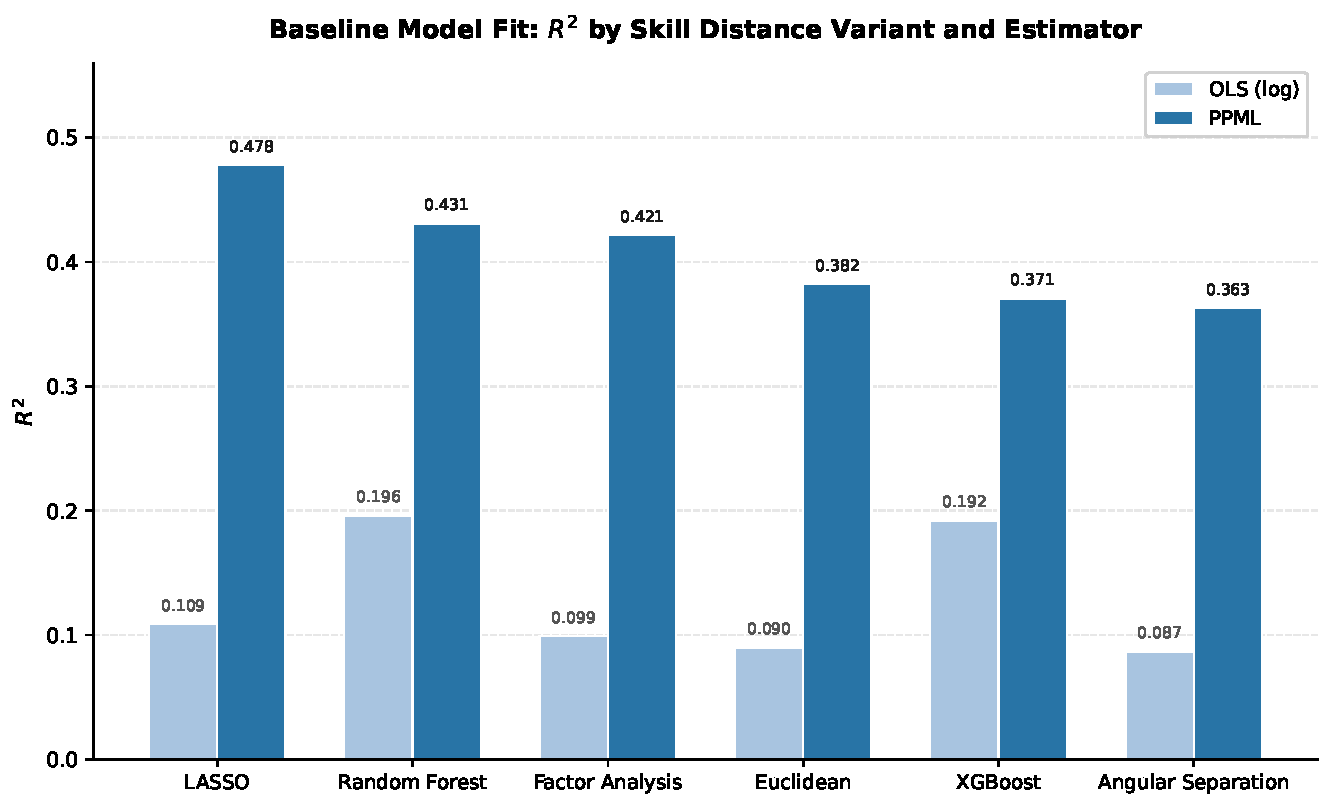
\includegraphics[width=0.85\textwidth]{fig_model_comparison.pdf}
\caption{Baseline model fit ($R^2$) by skill distance variant and estimator. PPML (dark) dominates OLS (light) across all variants. LASSO achieves the highest PPML $R^2$ (0.478).}
\label{fig:model_comparison}
\end{figure}

Three patterns emerge. First, PPML dominates OLS across all variants, with the best PPML specification ($R^2 = 0.478$) more than doubling the best OLS specification ($R^2 = 0.196$). This is expected: 95\% of pairs have zero switches, making the count structure naturally suited to PPML \citep{santos2006}. Second, ML-based skill distances outperform direct metrics under PPML, with LASSO achieving the highest $R^2$. LASSO retains 117 of 202 O*NET dimensions, effectively learning which dimensions matter for switching rather than treating all 202 equally. Factor analysis, the best direct metric at $R^2 = 0.421$, suggests that a few broad skill clusters capture most of the mobility-relevant variation. Third, geographic distance contributes substantial explanatory power: adding the Duncan index to the LASSO/PPML specification increases $R^2$ by 9.8 percentage points, and the increment is even larger for factor analysis (+14.3 pp). Workers switch to occupations that exist where they already live.

Figure \ref{fig:lasso_coefs} displays the 40 largest LASSO coefficients by magnitude, colored by O*NET descriptor category. The most influential dimensions span all four categories: Science (Knowledge), Assisting and Caring for Others (Work Activity), Computers and Electronics (Knowledge), Installation (Skill), and Written Expression (Ability). Negative coefficients indicate dimensions where greater between-occupation differences \emph{reduce} predicted switching; positive coefficients indicate dimensions where differences \emph{increase} it, potentially reflecting sorting toward complementary specializations.

\begin{figure}[H]
\centering
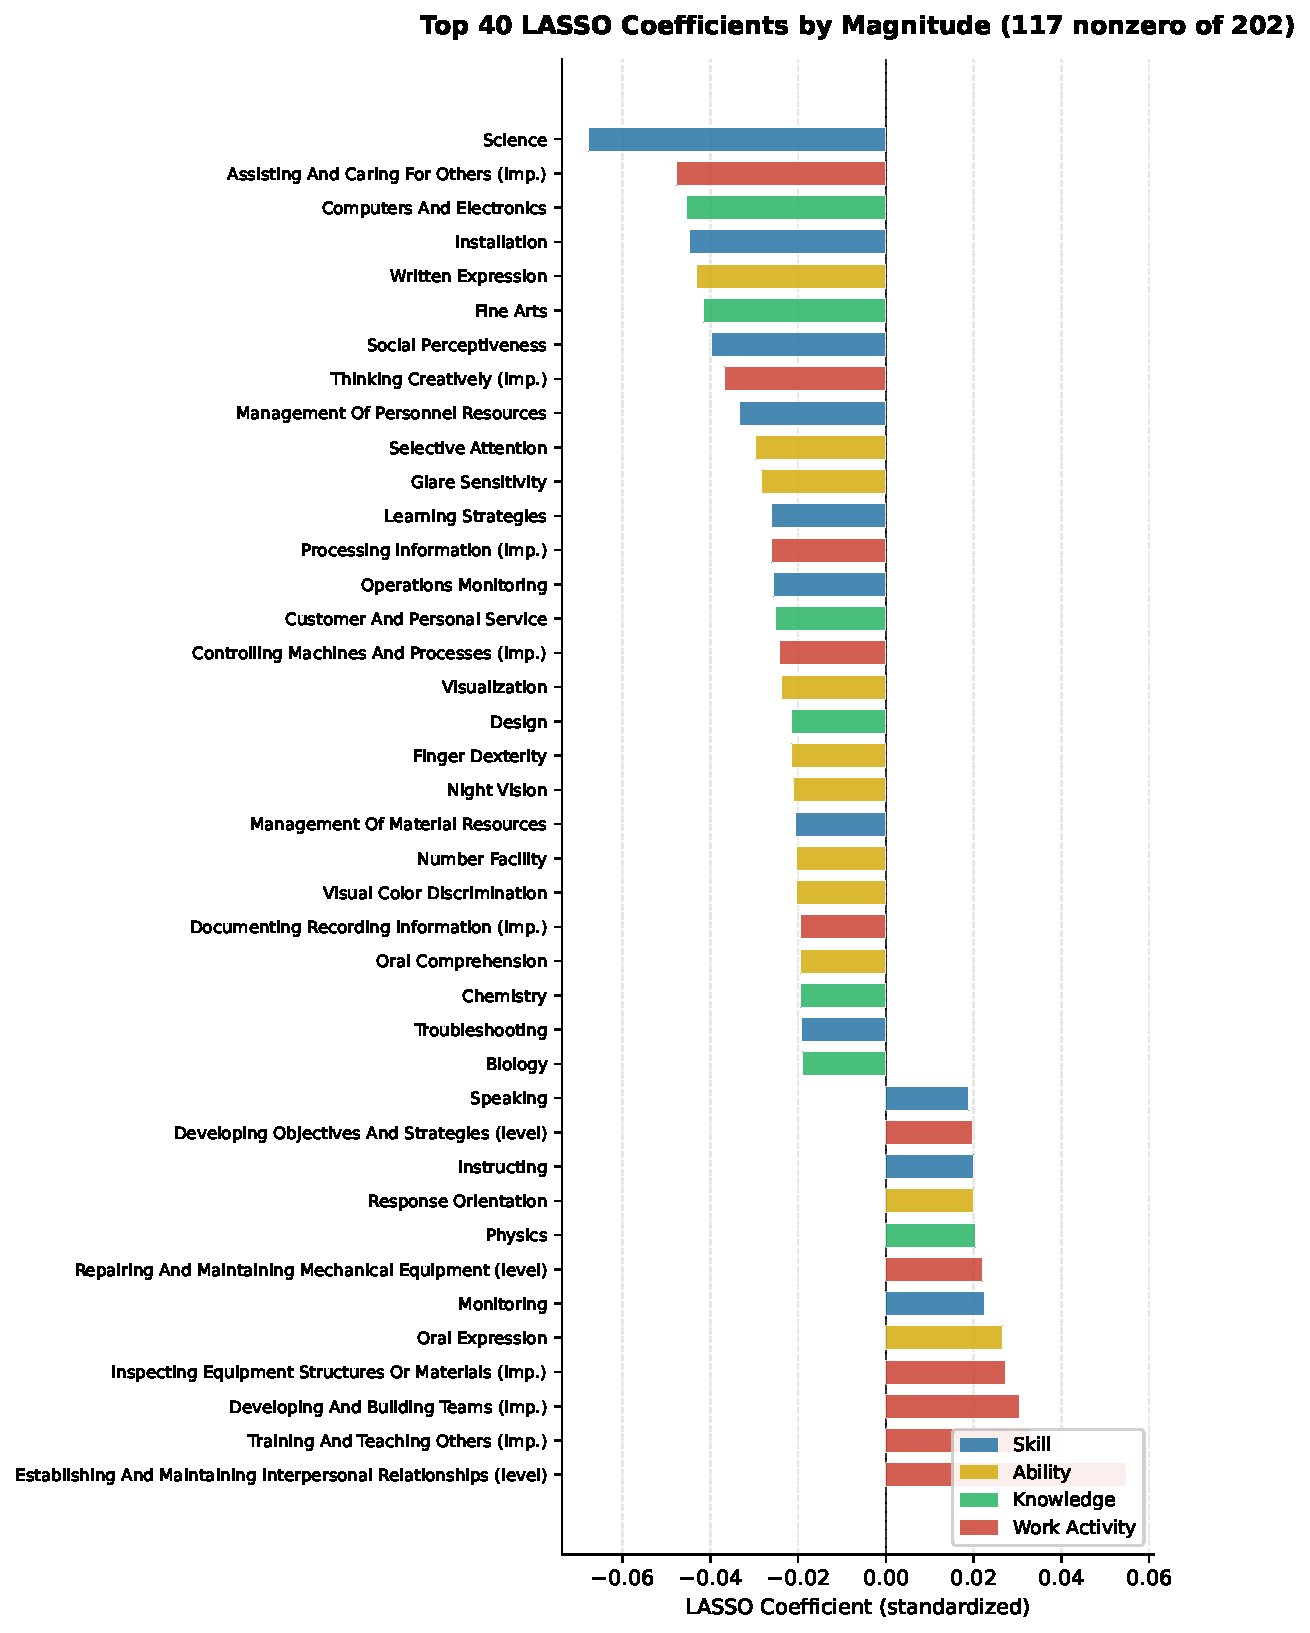
\includegraphics[width=\textwidth]{fig_lasso_coefficients.pdf}
\caption{Top 40 LASSO coefficients by magnitude (117 nonzero of 202). Bars are colored by O*NET descriptor category. Negative coefficients indicate that larger between-occupation differences on that dimension reduce predicted switching.}
\label{fig:lasso_coefs}
\end{figure}

All $\hat{\beta}_1$ coefficients are significant at $p < 0.001$ in every specification and every variant. The sign difference between direct and ML metrics is by construction: direct metrics measure dissimilarity (more distance $\rightarrow$ fewer switches, so $\hat{\beta}_1 < 0$), while ML metrics are predicted switches (higher prediction $\rightarrow$ more actual, so $\hat{\beta}_1 > 0$).

%-----------------------------------------------------------------------------
\subsection{Robustness Checks}
\label{sec:results_robust}
%-----------------------------------------------------------------------------

Four robustness checks confirm the stability of the baseline result:

\begin{enumerate}
    \item \textbf{Fixed $\delta_1 = 1$}: Entering total switches out as an exposure term rather than a free regressor tests whether results survive when the model explains switching \emph{rates} rather than levels. Skill distance remains significant ($p < 0.001$) in all variants. OLS $R^2$ rises to 0.276, reflecting the tighter specification.

    \item \textbf{Small-occupation removal}: Dropping occupations with fewer than 100 or 500 raw employment observations tests whether results are driven by noisy small-cell pairs. $\hat{\beta}_1$ is stable across thresholds. OLS $R^2$ increases slightly (the remaining pairs are better measured), while PPML $R^2$ decreases (fewer zero-pairs to explain).

    \item \textbf{Two-part model}: Separating the extensive margin (logit: does any switching occur?) from the intensive margin (OLS on positives: conditional on switching, how many?) shows that skill and geographic distance strongly predict \emph{whether} any switching occurs (logit pseudo-$R^2 = 0.222$ for factor analysis) but have less power over conditional magnitude ($R^2 = 0.127$), where idiosyncratic factors dominate.

    \item \textbf{Year fixed effects}: Estimating Equation (\ref{eq:switching}) on year-level switching data with year dummies absorbs COVID-era reshuffling and time trends. The pattern is identical: LASSO/PPML remains best ($R^2 = 0.411$), and skill distance is consistently significant.
\end{enumerate}

%-----------------------------------------------------------------------------
\subsection{Fixed-$\delta_1$ $R^2$ Comparison}
\label{sec:results_fixed}
%-----------------------------------------------------------------------------

Table \ref{tab:fixed_r2} reports the pseudo-$R^2$ under the fixed-$\delta_1$ exposure constraint for all six variants. This specification is used for index construction.

\begin{table}[H]
\centering
\caption{Fixed-$\delta_1$ PPML: $R^2$ Comparison Across Skill Distance Variants}
\label{tab:fixed_r2}
\begin{tabular}{lcccc}
\toprule
\textbf{Skill Distance} & \textbf{$R^2$ (fixed $\delta_1$)} & \textbf{$R^2$ (baseline)} & \textbf{$\hat{\beta}_1$} & \textbf{$p$-value} \\
\midrule
\textbf{LASSO}              & \textbf{0.326} & 0.478 & $+5.398$ & $<0.001$ \\
Random Forest               & 0.276          & 0.431 & $+0.445$ & $<0.001$ \\
Factor Analysis             & 0.265          & 0.421 & $-0.979$ & $<0.001$ \\
Euclidean                   & 0.212          & 0.382 & $-0.561$ & $<0.001$ \\
XGBoost                     & 0.201          & 0.371 & $+0.032$ & $<0.001$ \\
Angular Separation          & 0.188          & 0.363 & $-2.524$ & $<0.001$ \\
\bottomrule
\end{tabular}
\begin{minipage}{0.9\textwidth}
\vspace{0.5em}
\footnotesize \textit{Notes:} $N = 275{,}100$. Fixed $\delta_1$ is implemented by entering total switches out of origin as a PPML exposure term. The ranking of variants is preserved relative to the baseline: LASSO $>$ Random Forest $>$ Factor Analysis $>$ Euclidean $>$ XGBoost $>$ Angular Separation. $R^2$ declines uniformly because the exposure constraint is strictly more restrictive.
\end{minipage}
\end{table}

LASSO remains the best specification ($R^2 = 0.326$), preserving the baseline ranking. The $R^2$ decline relative to the baseline is uniform across variants, reflecting the cost of the exposure constraint. The key result is that the \emph{relative} ranking of variants is unchanged, confirming that the choice of preferred metric is robust to the exposure specification.

%-----------------------------------------------------------------------------
\subsection{Portability Index Rankings}
\label{sec:results_rankings}
%-----------------------------------------------------------------------------

Table \ref{tab:top_bottom} reports the 20 most and 20 least portable occupations under the fixed-$\delta_1$ LASSO/PPML specification with rank normalization.

\begin{table}[H]
\centering
\caption{Top 20 and Bottom 20 Occupations by Portability Index (LASSO, Fixed $\delta_1$)}
\label{tab:top_bottom}
\small
\begin{tabular}{rlcc}
\toprule
\textbf{Rank} & \textbf{Occupation} & \textbf{Index} & \textbf{PortRate} \\
\midrule
\multicolumn{4}{l}{\textit{Panel A: Most Portable}} \\
1  & Receptionists and information clerks          & 1.000 & 0.01251 \\
2  & Office clerks, general                        & 0.998 & 0.01213 \\
3  & Cashiers                                      & 0.996 & 0.01099 \\
4  & Laborers and freight, stock movers, hand       & 0.994 & 0.01075 \\
5  & Couriers and messengers                       & 0.992 & 0.00977 \\
6  & Stockers and order fillers                    & 0.990 & 0.00961 \\
7  & Retail salespersons                           & 0.989 & 0.00944 \\
8  & First-line supervisors of non-retail sales    & 0.987 & 0.00929 \\
9  & Customer service representatives              & 0.985 & 0.00927 \\
10 & Sales reps., wholesale and manufacturing      & 0.983 & 0.00901 \\
11 & Data entry keyers                             & 0.981 & 0.00869 \\
12 & Food service managers                         & 0.979 & 0.00845 \\
13 & Cooks                                         & 0.977 & 0.00833 \\
14 & Managers, all other                           & 0.975 & 0.00813 \\
15 & Waiters and waitresses                        & 0.973 & 0.00787 \\
16 & Secondary school teachers                     & 0.971 & 0.00785 \\
17 & Physical therapists                           & 0.969 & 0.00771 \\
18 & First-line supervisors, office/admin support  & 0.968 & 0.00764 \\
19 & Secretaries and administrative assistants     & 0.966 & 0.00758 \\
20 & Billing and posting clerks                    & 0.964 & 0.00739 \\
\midrule
\multicolumn{4}{l}{\textit{Panel B: Least Portable}} \\
506 & Engine and other machine assemblers          & 0.036 & 0.00026 \\
507 & Aircraft pilots and flight engineers         & 0.034 & 0.00026 \\
508 & Tire builders                                & 0.032 & 0.00024 \\
509 & Graders and sorters, agricultural products   & 0.031 & 0.00024 \\
510 & Furnace, kiln, oven, drier operators         & 0.029 & 0.00021 \\
511 & Bioengineers and biomedical engineers        & 0.027 & 0.00021 \\
512 & Derrick, rotary drill, service unit operators & 0.025 & 0.00020 \\
513 & Fishing and hunting workers                  & 0.023 & 0.00020 \\
514 & Proofreaders and copy markers                & 0.021 & 0.00020 \\
515 & Ship and boat captains and operators         & 0.019 & 0.00020 \\
516 & Millwrights                                  & 0.017 & 0.00020 \\
517 & Riggers                                      & 0.015 & 0.00019 \\
518 & Woodworking machine setters, operators       & 0.013 & 0.00018 \\
519 & Astronomers and physicists                   & 0.011 & 0.00018 \\
520 & Avionics technicians                         & 0.010 & 0.00017 \\
521 & Petroleum engineers                          & 0.008 & 0.00016 \\
522 & Actors                                       & 0.006 & 0.00016 \\
523 & Dancers and choreographers                   & 0.004 & 0.00015 \\
524 & Explosives workers, ordnance handling experts & 0.002 & 0.00015 \\
525 & Marine engineers and naval architects        & 0.000 & 0.00011 \\
\bottomrule
\end{tabular}
\begin{minipage}{0.9\textwidth}
\vspace{0.5em}
\footnotesize \textit{Notes:} Index is rank-normalized to $[0,1]$. PortRate is the employment-share-weighted predicted switching rate per switcher from the fixed-$\delta_1$ PPML model.
\end{minipage}
\end{table}

The top of the distribution is dominated by clerical, retail, food service, and general management occupations whose skill profiles overlap with many large destination sectors. The bottom is populated by highly specialized occupations with narrow skill profiles: petroleum engineers, marine engineers, avionics technicians, and similar niche occupations whose human capital does not generalize.

Figure \ref{fig:industry} shows the distribution of portability ranks across broad industry groups, confirming the expected pattern: Education and Business/Office occupations cluster at high portability, while STEM, Skilled Trades, and Production/Transport occupations are concentrated at lower portability ranks with wider dispersion.

\begin{figure}[H]
\centering
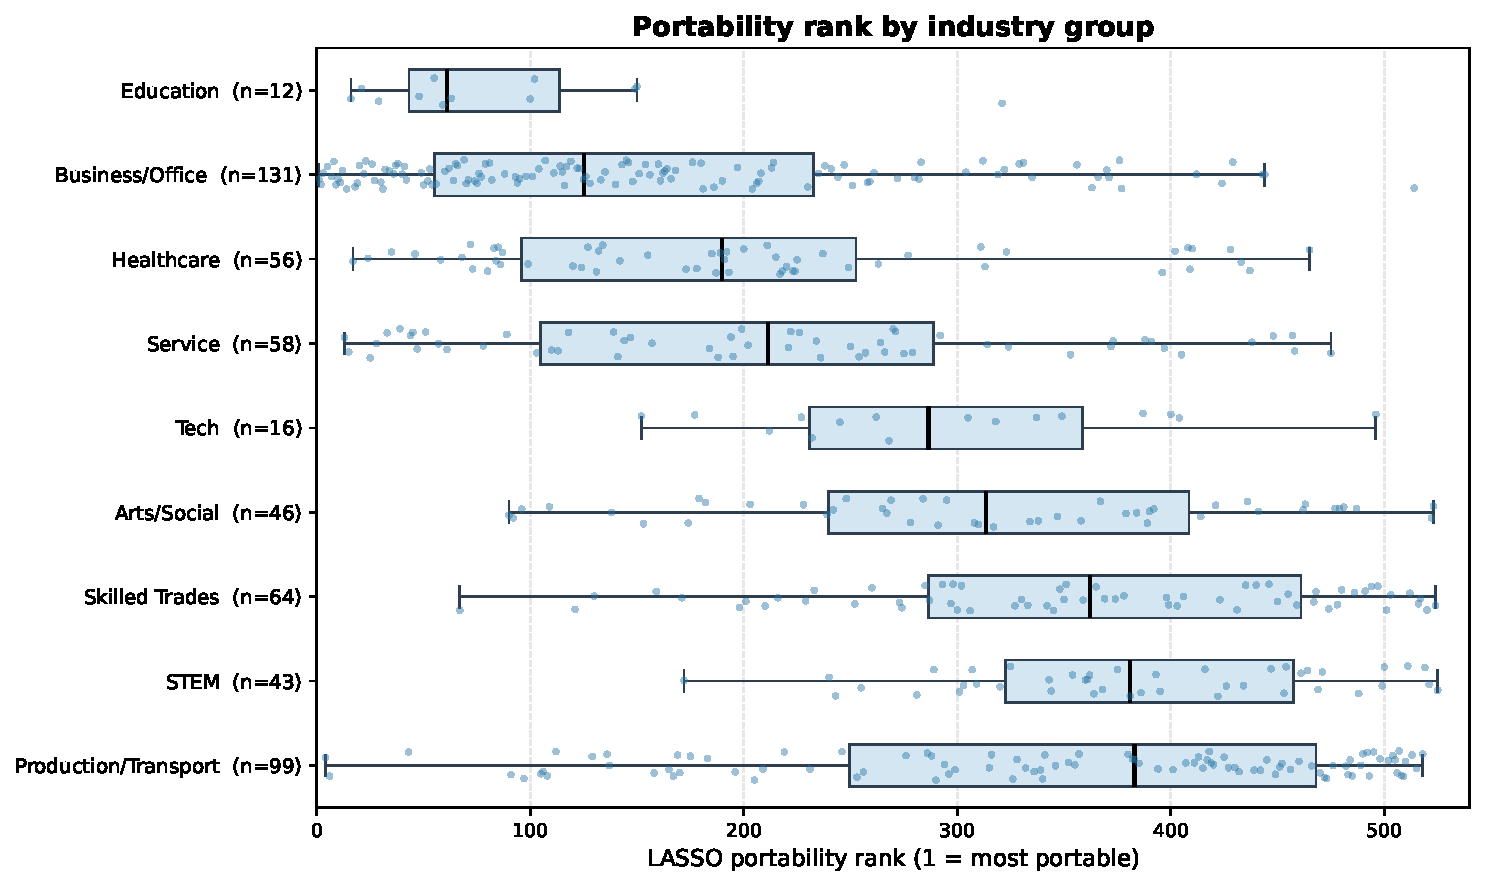
\includegraphics[width=\textwidth]{fig_portability_by_industry.pdf}
\caption{Portability rank by industry group. Lower rank = more portable. Box plots show median, interquartile range, and individual occupations (dots). Education and Business/Office occupations are the most portable; STEM and Production/Transport are the least.}
\label{fig:industry}
\end{figure}

Table \ref{tab:notable} reports selected occupations of substantive interest, comparing the fixed-$\delta_1$ index with the earlier per-worker baseline.

\begin{table}[H]
\centering
\caption{Notable Occupations: Fixed-$\delta_1$ Index vs.\ Per-Worker Baseline}
\label{tab:notable}
\begin{tabular}{lccc}
\toprule
\textbf{Occupation} & \textbf{Index} & \textbf{Rank (of 525)} & \textbf{Per-Worker Rank} \\
\midrule
Software developers          & 0.490 & 268 & 519 \\
Registered nurses             & 0.527 & 249 & 516 \\
Electricians                  & 0.242 & 398 & 521 \\
Mechanical engineers          & 0.149 & 447 & 518 \\
Aerospace engineers           & 0.048 & 500 & 524 \\
Aircraft pilots               & 0.034 & 507 & 522 \\
Petroleum engineers           & 0.008 & 521 & 523 \\
\bottomrule
\end{tabular}
\begin{minipage}{0.9\textwidth}
\vspace{0.5em}
\footnotesize \textit{Notes:} Per-worker rank is based on the per-million-worker portability rate from the free-$\delta_1$ specification. The fixed-$\delta_1$ index substantially improves the ranking of software developers (519 $\to$ 268) and registered nurses (516 $\to$ 249) by stripping origin-size contamination.
\end{minipage}
\end{table}

Software developers and registered nurses move from the very bottom of the per-worker ranking ($\sim$519 and $\sim$516 of 525) to near the median of the fixed-$\delta_1$ index (268 and 249). The fixed-$\delta_1$ specification recognizes that these occupations' skill profiles are structurally close to many large destinations, even though observed switching volume is low, either because workers in these occupations are well-compensated (reducing voluntary mobility) or because institutional barriers suppress transitions. Aerospace engineers, pilots, and petroleum engineers remain near the bottom in both measures, consistent with genuinely narrow skill profiles.

%-----------------------------------------------------------------------------
\subsection{Factor Analysis vs.\ LASSO: Licensing Frictions}
\label{sec:results_factor}
%-----------------------------------------------------------------------------

Both the factor-analysis and LASSO indices are constructed identically (fixed $\delta_1 = 1$, employment-share-weighted rate, rank-normalized), with the only difference being the underlying skill-distance measure. The Spearman rank correlation between the two indices is $\rho = 0.890$, indicating broad agreement. However, the indices diverge sharply for specific occupations, and the pattern of divergence is substantively informative.

Table \ref{tab:factor_lasso} reports occupations with the largest rank differences.

\begin{table}[H]
\centering
\caption{Factor Analysis vs.\ LASSO Portability: Notable Rank Differences}
\label{tab:factor_lasso}
\begin{tabular}{lcccc}
\toprule
\textbf{Occupation} & \textbf{Factor Rank} & \textbf{LASSO Rank} & \textbf{$\Delta$ Rank} & \textbf{Licensed?} \\
\midrule
Registered nurses             & 47  & 249 & $+202$ & Yes \\
Electricians                  & 95  & 398 & $+303$ & Yes \\
Aircraft pilots               & 402 & 507 & $+105$ & Yes \\
Hairdressers/cosmetologists   & 8   & 118 & $+110$ & Yes \\
Farmers/ranchers              & 384 & 443 & $+59$  & Partial \\
Mechanical engineers          & 404 & 447 & $+43$  & Partial \\
Teaching assistants            & 13  & 48  & $+35$  & No \\
Secondary school teachers     & 1   & 16  & $+15$  & Yes \\
Software developers           & 306 & 268 & $-38$  & No \\
Aerospace engineers           & 495 & 500 & $+5$   & No \\
Petroleum engineers           & 521 & 521 & $0$    & No \\
\bottomrule
\end{tabular}
\begin{minipage}{0.9\textwidth}
\vspace{0.5em}
\footnotesize \textit{Notes:} $\Delta$ Rank = Factor rank $-$ LASSO rank. Positive values indicate the occupation is rated more portable under factor analysis. ``Licensed?'' is based on common regulatory requirements for these occupations. The two indices agree almost perfectly at the extremes (petroleum engineers: rank 521 in both) but diverge sharply for credentialed occupations.
\end{minipage}
\end{table}

Figure \ref{fig:rank_scatter} plots factor-analysis ranks against LASSO ranks for all 525 occupations, with points colored by occupational licensing share. Occupations above the 45-degree line are rated more portable under factor analysis than LASSO. The licensed occupations (red-shaded points) systematically appear above the line, visualizing the licensing friction gap.

\begin{figure}[H]
\centering
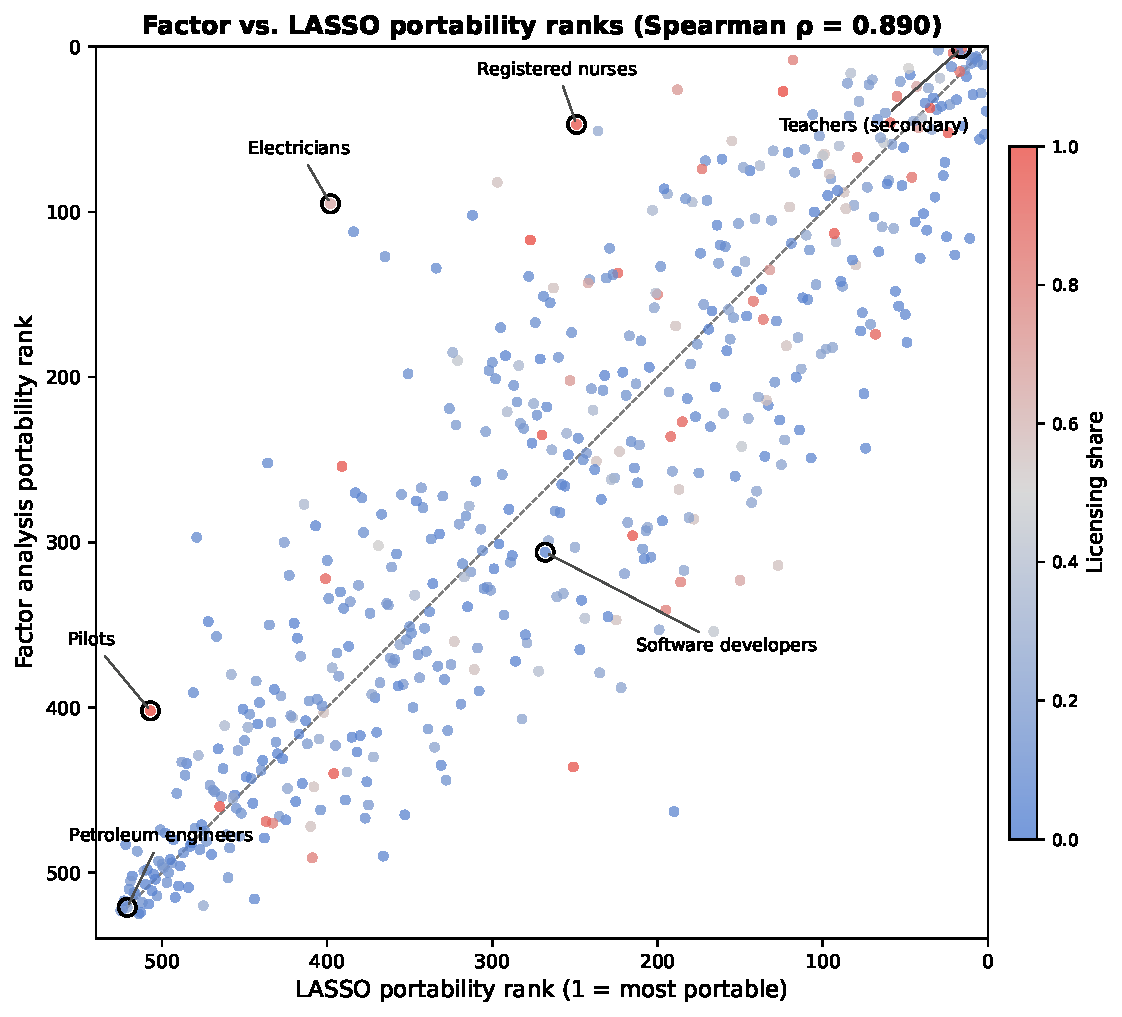
\includegraphics[width=0.85\textwidth]{fig_rank_scatter.pdf}
\caption{Factor analysis vs.\ LASSO portability ranks ($N = 525$). Points above the 45-degree line are rated more portable under factor analysis. Color indicates licensing share (red = licensed). Licensed occupations (nurses, electricians, pilots) systematically diverge above the line, consistent with licensing frictions suppressing observed mobility.}
\label{fig:rank_scatter}
\end{figure}

The largest movers are registered nurses (+202 ranks) and electricians (+303 ranks). Under factor analysis, these occupations' broad latent-skill profiles (interpersonal, analytical, and physical dimensions that overlap with many large destinations) are recognized as structurally transferable. Under LASSO, they are penalized because observed switching in the CPS is suppressed by licensing and credentialing barriers.

The interpretation is that factor analysis captures \emph{structural portability}, the latent skill overlap that could support transitions absent institutional barriers, while LASSO captures \emph{revealed portability}, the skill dimensions that predict transitions that actually occur. The divergence maps onto licensing frictions \citep{kleiner2013}: nurses, electricians, hairdressers, and pilots are all subject to state-level licensing requirements that raise the cost of occupational entry, suppressing observed switching despite underlying skill compatibility.

Software developers are one of the few occupations that score higher under LASSO than factor analysis ($-38$ ranks). This may reflect that the specific dimensions LASSO selects (technical problem-solving, data analysis) are shared with many large destination occupations, even though the four-factor latent representation places software developers in a more specialized cluster.

%-----------------------------------------------------------------------------
\subsection{Equation 7: Long-Term Unemployment Validation}
\label{sec:results_ltu}
%-----------------------------------------------------------------------------

Table \ref{tab:ltu} reports results from Equation (\ref{eq:ltu}) and its extensions.

\begin{table}[H]
\centering
\caption{Portability and Long-Term Unemployment: Equation 7 Results}
\label{tab:ltu}
\begin{tabular}{llcccc}
\toprule
\textbf{Model} & \textbf{Variable} & \textbf{Coef.} & \textbf{SE} & \textbf{$p$} & \textbf{$R^2$} \\
\midrule
\multirow{2}{*}{1. Baseline (free $\delta_1$)} & EmpTrend & $+0.0001$ & 0.0002 & 0.279 & \multirow{2}{*}{0.003} \\
 & Portability & $+0.0001$ & 0.0002 & 0.279 & \\
\midrule
\multirow{2}{*}{2. Full (fixed $\delta_1$)} & EmpTrend$_z$ & $+0.0004$ & 0.0010 & 0.700 & \multirow{2}{*}{0.020} \\
 & Portability$_z$ & $\mathbf{-0.0011}$ & 0.0004 & $\mathbf{0.008}$ & \\
\midrule
3. Portability only & Portability$_z$ & $-0.0011$ & 0.0004 & 0.008 & 0.018 \\
\midrule
\multirow{3}{*}{4. AI additive} & EmpTrend$_z$ & $+0.0003$ & 0.0010 & 0.755 & \multirow{3}{*}{0.026} \\
 & Portability$_z$ & $\mathbf{-0.0009}$ & 0.0004 & $\mathbf{0.035}$ & \\
 & AI$_z$ & $-0.0006$ & 0.0004 & 0.078 & \\
\midrule
\multirow{4}{*}{5. AI interaction} & EmpTrend$_z$ & $+0.0003$ & 0.0010 & 0.740 & \multirow{4}{*}{0.027} \\
 & Portability$_z$ & $-0.0009$ & 0.0004 & 0.036 & \\
 & AI$_z$ & $-0.0007$ & 0.0004 & 0.062 & \\
 & Port.$\times$AI & $-0.0002$ & 0.0005 & 0.705 & \\
\bottomrule
\end{tabular}
\begin{minipage}{0.9\textwidth}
\vspace{0.5em}
\footnotesize \textit{Notes:} $N = 524$ occupations. LTU is the share of unemployed workers (last occupation $= o$) with $\geq$26 weeks of unemployment. All continuous regressors are z-scored. Model 1 uses the free-$\delta_1$ portability measure. Models 2--5 use the fixed-$\delta_1$ (Option C) portability index. 95\% CI for $\hat{\alpha}_2$ in Model 2: $[-0.0019, -0.0003]$.
\end{minipage}
\end{table}

Figure \ref{fig:portability_ltu} presents the partial regression plot corresponding to Model 2, with both portability and LTU residualized on the employment trend. The negative slope ($\hat{\alpha}_2 = -0.0011$, $p = 0.008$) is visually apparent despite substantial noise, and notable occupations are labeled for reference.

\begin{figure}[H]
\centering
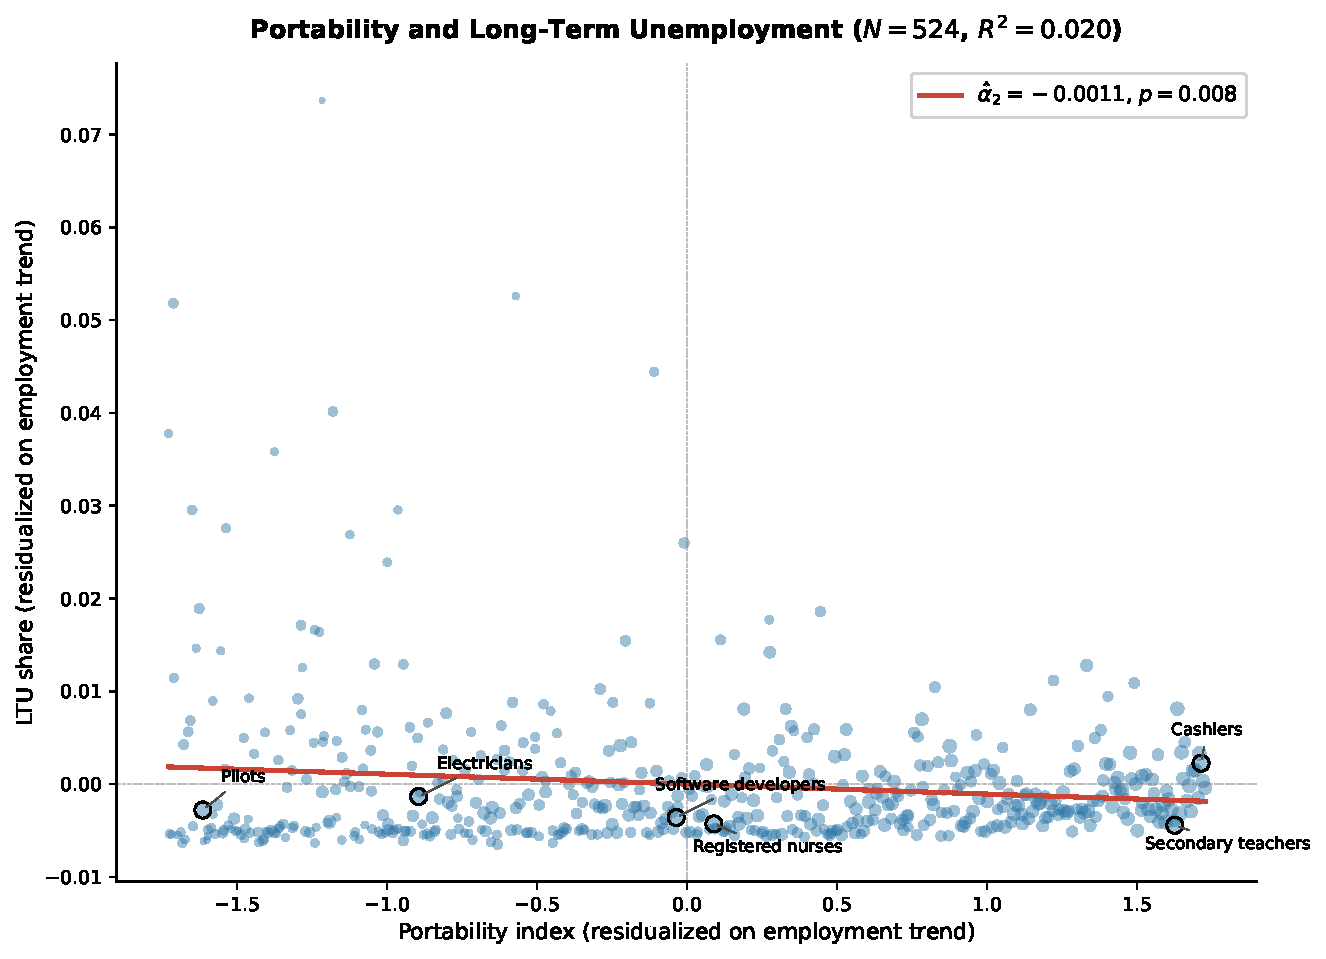
\includegraphics[width=0.85\textwidth]{fig_portability_ltu.pdf}
\caption{Portability and long-term unemployment ($N = 524$). Both axes are residualized on the employment trend control. The fitted line shows $\hat{\alpha}_2 = -0.0011$ ($p = 0.008$): more portable occupations have lower LTU shares. Selected occupations are labeled.}
\label{fig:portability_ltu}
\end{figure}

The key result is the transition from Model 1 to Model 2. Under the free-$\delta_1$ portability measure, the coefficient on portability is positive (wrong sign) and insignificant ($p = 0.279$, $R^2 = 0.003$). Under the fixed-$\delta_1$ index, the coefficient flips to $-0.0011$ and becomes significant at $p = 0.008$, with the entire 95\% confidence interval below zero ($[-0.0019, -0.0003]$). A one-standard-deviation increase in portability reduces the LTU share by 0.11 percentage points. The sign flip underscores the importance of stripping origin-size contamination: the free-$\delta_1$ measure was dominated by a ``big occupation'' artifact that reversed the structural relationship.

%-----------------------------------------------------------------------------
\subsection{AI Exposure Results}
\label{sec:results_ai}
%-----------------------------------------------------------------------------

Models 4 and 5 in Table \ref{tab:ltu} add AI exposure from \citet{eloundou2023}. Three findings emerge:

\begin{enumerate}
    \item \textbf{Portability survives conditioning on AI exposure.} In Model 4, portability remains significant at $p = 0.035$ ($\hat{\alpha}_2 = -0.0009$). The coefficient attenuates slightly from the baseline ($-0.0011$ to $-0.0009$) but remains economically and statistically meaningful. The portability--LTU relationship is not confounded by AI exposure differences across occupations.

    \item \textbf{AI exposure is marginally significant with a negative sign.} Higher AI-exposed occupations have \emph{lower} LTU ($\hat{\alpha}_3 = -0.0006$, $p = 0.078$). This is counterintuitive if one expects AI-exposed occupations to suffer displacement, but consistent with AI-exposed jobs being disproportionately white-collar, cognitive occupations with structurally low baseline unemployment.

    \item \textbf{The interaction term is null.} In Model 5, the portability $\times$ AI interaction is insignificant ($p = 0.705$), meaning portability's effect on LTU does not vary by AI exposure level. The hypothesis that ``portability buffers AI displacement'' is not supported. Subsample splits by median AI exposure (not shown) confirm this: portability coefficients are similar in magnitude ($\sim$$-0.0008$) but insignificant in both halves ($p = 0.177$ and $p = 0.160$), likely reflecting a power issue with only 262 observations per subsample.
\end{enumerate}

The bottom line for interpretation: portability and AI exposure operate through independent channels. Higher portability predicts lower LTU regardless of AI exposure level.

%=============================================================================
\section{Discussion}
\label{sec:discussion}
%=============================================================================

%-----------------------------------------------------------------------------
\subsection{Why Do Some High-Skilled Occupations Score Low?}
%-----------------------------------------------------------------------------

The portability index reflects \emph{breadth} of outside options weighted by destination size, not the \emph{quality} of human capital. Occupations like aerospace engineering and petroleum engineering score low because their skill profiles overlap primarily with small, specialized destination sectors. The employment-share weighting in Equation (\ref{eq:portrate}) penalizes narrow-but-high-value destinations: being structurally close to 10 small engineering niches counts less than being close to one large service sector.

This connects to \citeauthor{lazear2009}'s (\citeyear{lazear2009}) theory of skill specificity. In Lazear's framework, occupations that combine skills in rare proportions are ``specific'' not because their component skills are unusual, but because the particular combination is. An aerospace engineer may have high levels of mathematics, physics, and project management, all individually common, but the specific blend is rare, making the occupation's skill \emph{bundle} non-portable even though each component skill is individually transferable. The portability index captures this distinction: it measures bundle transferability, not component-skill value.

%-----------------------------------------------------------------------------
\subsection{Licensing Frictions as a Key Finding}
%-----------------------------------------------------------------------------

The comparison of factor-analysis and LASSO indices is arguably the paper's most novel finding. The two measures agree at the extremes (petroleum engineers score identically at rank 521/521, and general clerical occupations dominate both tops) but diverge dramatically in the middle, precisely where institutional barriers are most binding.

Factor analysis measures \emph{structural portability}: the latent skill overlap between occupations, computed from the full 202-dimensional O*NET profile compressed into four factors. It answers the question ``how similar are these occupations' skill requirements?'' without reference to whether workers actually transition between them. LASSO measures \emph{revealed portability}: the skill dimensions that predict observed transitions in the CPS data. It answers the question ``which skill differences predict who actually switches?''

The divergence for licensed occupations (nurses +202 ranks, electricians +303 ranks, hairdressers +110 ranks, pilots +105 ranks) is interpretable as the \emph{licensing friction gap}. These occupations have broad skill profiles that should, in principle, support transitions to many destinations. But state-level licensing requirements raise the cost of entry, suppressing the observed switching that LASSO uses as its training signal. Factor analysis, by contrast, sees only the latent skill structure and rates these occupations as highly portable.

This finding connects to the licensing literature \citep{kleiner2013}: occupational licensing affects approximately 25\% of U.S.\ workers, and licensing requirements are a binding constraint on labor mobility for many middle-skill occupations. The comparison of factor-analysis and LASSO indices provides a new way to quantify the \emph{mobility suppression} effect of licensing, not by comparing licensed vs.\ unlicensed workers directly, but by comparing two portability measures that differ only in whether they condition on observed switching.

%-----------------------------------------------------------------------------
\subsection{Limitations}
%-----------------------------------------------------------------------------

Several limitations warrant discussion.

\paragraph{CPS occupation coding error.} The 12.5\% individual-level switching rate is roughly double the 5\% benchmark established by careful longitudinal studies \citep{kambourov2008}. Much of the excess likely reflects coding error: respondents describe their occupations differently in consecutive surveys, generating spurious switches. This measurement error adds noise to the dependent variable and attenuates the signal from skill distance, making our estimates conservative. However, if coding error is systematically related to skill distance (e.g., similar occupations are more likely to be miscoded as each other), the estimates could be biased toward finding an effect.

\paragraph{Single time window.} The switching data span 2020--2025, a period that includes the COVID-19 pandemic, the ``great resignation,'' and subsequent labor market tightening. Year fixed effects confirm that the baseline patterns are stable within this window, but the model is estimated on a single historical period and may not generalize to other macroeconomic environments.

\paragraph{Descriptive, not causal.} The LTU regression (Equation \ref{eq:ltu}) is a cross-sectional correlation between an occupation-level portability index and an occupation-level LTU share. There is no quasi-experimental variation or instrumental variable; the employment trend control absorbs some confounds but cannot establish causality. The result should be interpreted as ``occupations with more portable skill profiles tend to have lower LTU,'' not ``making skills more portable would reduce LTU.''

\paragraph{ACS 2021 vs.\ specification's 2023.} The geographic distance matrix uses ACS 2021 instead of the specified 2023 reference year, due to the PUMA vintage incompatibility described in Section \ref{sec:data_geo}. Geographic employment distributions evolve slowly, but this deviation introduces a two-year lag.

\paragraph{No out-of-sample validation.} The portability index is constructed from the full 2020--2025 sample. A train-test temporal split (e.g., train on 2020--2024, validate on 2025) would provide a stronger test of the index's predictive validity but is not yet implemented.

\paragraph{Untapped O*NET dimensions.} The current pipeline uses 202 numeric dimensions from four O*NET descriptor files. O*NET also contains 18,796 free-text task statements, 2,087 Detailed Work Activities (DWAs), and 332 Intermediate Work Activities (IWAs) that could provide complementary measures of occupational similarity, particularly for distinguishing occupations that share the same broad skill levels but differ in what workers actually \emph{do}.

%=============================================================================
\section{Conclusion}
\label{sec:conclusion}
%=============================================================================

This paper makes three contributions. First, I construct a validated skill portability index for 525 U.S.\ occupations, demonstrating that LASSO-selected skill dimensions from O*NET predict bilateral switching flows substantially better than traditional distance metrics (pseudo-$R^2 = 0.478$ vs.\ best direct metric $R^2 = 0.421$). Second, I show that the fixed-exposure portability index significantly predicts long-term unemployment across occupations ($p = 0.008$), providing downstream validation of the measure. Third, the comparison of factor-analysis and LASSO indices reveals a systematic divergence for licensed occupations, offering a new lens on how credentialing requirements suppress observed mobility despite underlying skill compatibility.

The policy implication is that portability indices based on revealed switching behavior systematically understate the transferability of credentialed occupations. A nurse or electrician whose licensing requirements prevent them from switching, despite having skills that would transfer, appears ``non-portable'' in revealed-preference measures, potentially misleading workforce development programs that use such measures to identify at-risk workers. The structural measure based on factor analysis provides a complementary view, capturing the latent transferability that licensing suppresses.

The index is a tool, not a final answer. Its value depends on downstream use in workforce policy, retraining program design, or displacement risk assessment. Future work should validate the factor-vs.-LASSO divergence against direct licensing data \citep{kleiner2013}, compute bootstrap confidence intervals on the rank index, extend the measure to incorporate wage-preserving portability (whether outside options are not just accessible but economically viable), and explore cluster-aware index construction that accounts for the correlation structure of destination occupations.

%=============================================================================
% Bibliography
%=============================================================================

\begin{thebibliography}{99}

\bibitem[Autor et al.(2013)]{autor2013}
Autor, D. H., Dorn, D., \& Hanson, G. H. (2013).
The China syndrome: Local labor market effects of import competition in the United States.
\textit{American Economic Review}, 103(6), 2121--2168.

\bibitem[Becker(1964)]{becker1964}
Becker, G. S. (1964).
\textit{Human Capital: A Theoretical and Empirical Analysis, with Special Reference to Education}.
University of Chicago Press.

\bibitem[Cortes \& Gallipoli(2018)]{cortes2018}
Cortes, G. M., \& Gallipoli, G. (2018).
The costs of occupational mobility: An aggregate analysis.
\textit{Journal of the European Economic Association}, 16(2), 275--315.

\bibitem[Dorn(2009)]{dorn2009}
Dorn, D. (2009).
\textit{Essays on inequality, spatial interaction, and the demand for skills}.
Doctoral dissertation, University of St.\ Gallen.

\bibitem[Eloundou et al.(2023)]{eloundou2023}
Eloundou, T., Manning, S., Mishkin, P., \& Rock, D. (2023).
GPTs are GPTs: An early look at the labor market impact potential of large language models.
\textit{arXiv preprint arXiv:2303.10130}.

\bibitem[Gathmann \& Sch\"{o}nberg(2010)]{gathmann2010}
Gathmann, C., \& Sch\"{o}nberg, U. (2010).
How general is human capital? A task-based approach.
\textit{Journal of Labor Economics}, 28(1), 1--49.

\bibitem[Kambourov \& Manovskii(2008)]{kambourov2008}
Kambourov, G., \& Manovskii, I. (2008).
Rising occupational and industry mobility in the United States: 1968--97.
\textit{International Economic Review}, 49(1), 41--79.

\bibitem[Kleiner \& Krueger(2013)]{kleiner2013}
Kleiner, M. M., \& Krueger, A. B. (2013).
Analyzing the extent and influence of occupational licensing on the labor market.
\textit{Journal of Labor Economics}, 31(S1), S173--S202.

\bibitem[Lazear(2009)]{lazear2009}
Lazear, E. P. (2009).
Firm-specific human capital: A skill-weights approach.
\textit{Journal of Political Economy}, 117(5), 914--940.

\bibitem[Poletaev \& Robinson(2008)]{poletaev2008}
Poletaev, M., \& Robinson, C. (2008).
Human capital specificity: Evidence from the Dictionary of Occupational Titles and Displaced Worker Surveys, 1984--2000.
\textit{Journal of Labor Economics}, 26(3), 387--420.

\bibitem[Santos Silva \& Tenreyro(2006)]{santos2006}
Santos Silva, J. M. C., \& Tenreyro, S. (2006).
The log of gravity.
\textit{Review of Economics and Statistics}, 88(4), 641--658.

\bibitem[Shaw(1987)]{shaw1987}
Shaw, K. L. (1987).
Occupational change, employer change, and the transferability of skills.
\textit{Southern Economic Journal}, 53(3), 702--719.

\bibitem[Tolbert \& Sizer(1996)]{tolbert1996}
Tolbert, C. M., \& Sizer, M. (1996).
U.S.\ commuting zones and labor market areas: A 1990 update.
Economic Research Service Staff Paper No.\ 9614.

\end{thebibliography}

\end{document}
